\chapter{引言}

深度学习(Deep Learning)已经在许多机器学习任务上取得了巨大进展:物体识别\cite{krizhevsky2012imagenet}、目标检测\cite{redmon2016you}、语音识别\cite{saon2015ibm}、语言翻译\cite{sutskever2014sequence}、社交网络分类\cite{thomax2017semisupervised}等。在大数据和硬件加速的驱动下, 未经加工的特征可以被深度网络用更高级和更抽象地特征表示出来,减轻了传统机器学习方法中对手工设计的特征和专家知识的依赖,并在众多任务上取得了更好的性能。

深度学习技术正在走进并改变着人类生活的方方面面,世界上越来越多的应用和系统被其所赋能。例如,Google、 Telsa、 Uber等公司正在测试的自动驾驶汽车,它需要用到物体识别、目标检测、强化学习等大量现代深度学习驱动的技术。作为一种生物认证的方式,人脸识别系统被应用到移动设备的解锁、自助取款机、火车站安检机等处,甚至被执法部门用来追捕嫌疑犯。一些基于行为的恶意软件检测和异常检测解决方案也利用深度学习来寻找语义特征\cite{saxe2015deep}。

深度神经网络(Deep Neural Network, DNN)在具有强大的拟合能力且在许多任务上都表现出较好的泛化性能。即使模型的参数数量远远大于训练样本数(即过参数化),也没有出现严重的过拟合问题;即使模型优化时高度非凸、非光滑的损失函数并不能被保证找到全局最优解,也可以在工程应用中放心大胆的使用局部最优解;即使模型的可解释性差,也没有阻挡学术界和工业界将它视为一个黑盒广泛研究和应用。

成也萧何,败也萧何。近年来,通过反向传播学习到的深度神经网络被发现具有一个反直觉的特性和内在的盲点:即使一个在正常场景下表现良好的深度模型,也非常容易被精心设计的样本所欺骗,而这些样本对人类的感知系统来说却与正常样本无异\cite{goodfellow2014explaining},如\autoref{fig:adversarial_example}所示。Szegedy等人首先在图片上加入一些微小的扰动,使得最先进的做图片分类任务的深度神经网络能够以较大的概率被欺骗,即样本被错误分类。这些被错分类的恶意设计的样本被称为对抗样本(Adversarial examples)\cite{szegedy2013intriguing}。大量的基于深度学习技术的系统已经在现实世界被应用,或正在计划着去应用。同时,最近的研究表明,对抗样本也可以被应用到现实世界中。 例如,一个敌人通过对公路上的停车标志进行一些人类察觉不到的微小改动,便可
以迷惑自动驾驶汽车的交通信号识别系统, 使其无视停车信号标志\cite{kurakin2016adversarial, Eykholt_2018_CVPR};也可以通过类似的方式构造对抗样本,使得目标检测系统无法检测出路上的行人\cite{xie2017adversarial}。 攻击者也可以生成对抗指令去欺骗被应用到 Apple Siri、 Amazon Alexa、 Microsoft Cortana 上面的语音识别模型\cite{carlini2016hidden, zhang2017dolphinattack}。

\begin{figure}[h]
    \centering
    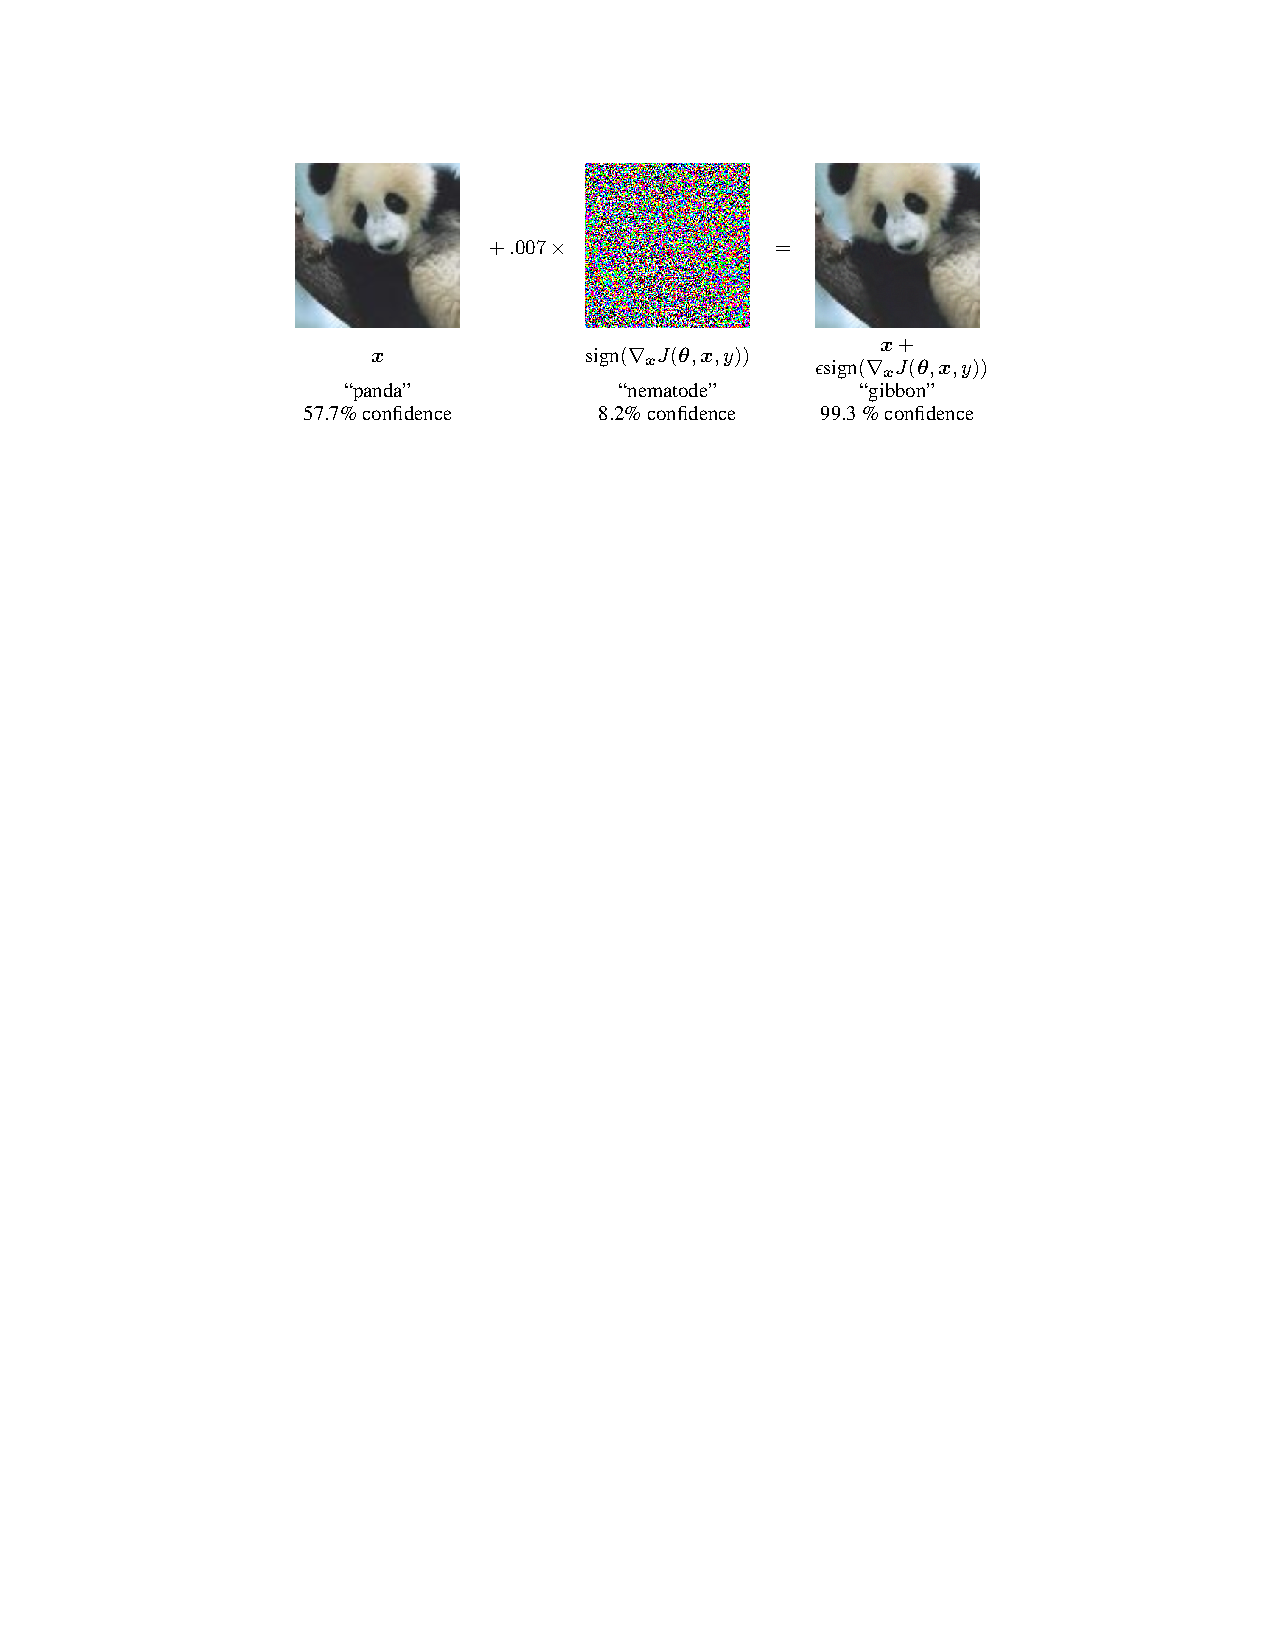
\includegraphics{fig/adversarial_example.pdf}
    \caption{对抗样本的一个演示,干净的样本能够被GoogLeNet\cite{szegedy2015going}正确识别成熊猫(Panda),而添加了不可察觉的扰动的对抗样本却被识别成了长臂猿(Gibbon)。左边:干净样本;中间:扰动;右边:对抗样本。}
    \label{fig:adversarial_example}
\end{figure}

在对抗样本的攻击下,深度神经网络表现出了非常差的鲁棒性,使得应用深度学习的系统都不可避免地存在着潜在的风险,尤其是在安全性非常重要的任务上。另一方面,深度神经网络如此反直觉的特性,让我们不得不反思:那些号称在某项任务上深度学习模型超越人类水平的标语真的有意义吗?那些深度网络的智能水平真的比得上人类智能吗?从对抗鲁棒性的语境下看,答案当然是否定的。对抗鲁棒性问题如此具有现实意义,同时又带有一定的哲学内涵,吸引了学者们前赴后继地进行研究,大量的防御方法被提出来,目的是为了能够让智能系统正确地认知对抗样本\cite{szegedy2013intriguing, gu2014towards, madry2018towards, papernot2016distillation, rozsa2016adversarial, zheng2016improving}。 然而,这些被提出来的防御措施大部分都不够有效,它们可以被更强大的敌人成功攻击\cite{carlini2017towards}。同时也有一些工作旨在验证和训练可证明鲁棒的神经网络,但是这些方法只能提供单点的保证,而且它们需要巨大的计算代价, 因此无法被推广到更为现实的数据集中\cite{raghunathan2018certified, pmlr-v80-wong18a, wong2018scaling}。 另外,基于检测的防御方法也被大量地提出来\cite{grosse2017statistical, gong2017adversarial, metzen2017detecting, li2017adversarial, feinman2017detecting},然而, Carlini 和 Wagner的研究\cite{carlini2017adversarial}表明这些防御措施都可以被使用具有针对性的攻击机制的敌人轻易地规避。

\begin{figure}[h]
    \centering
    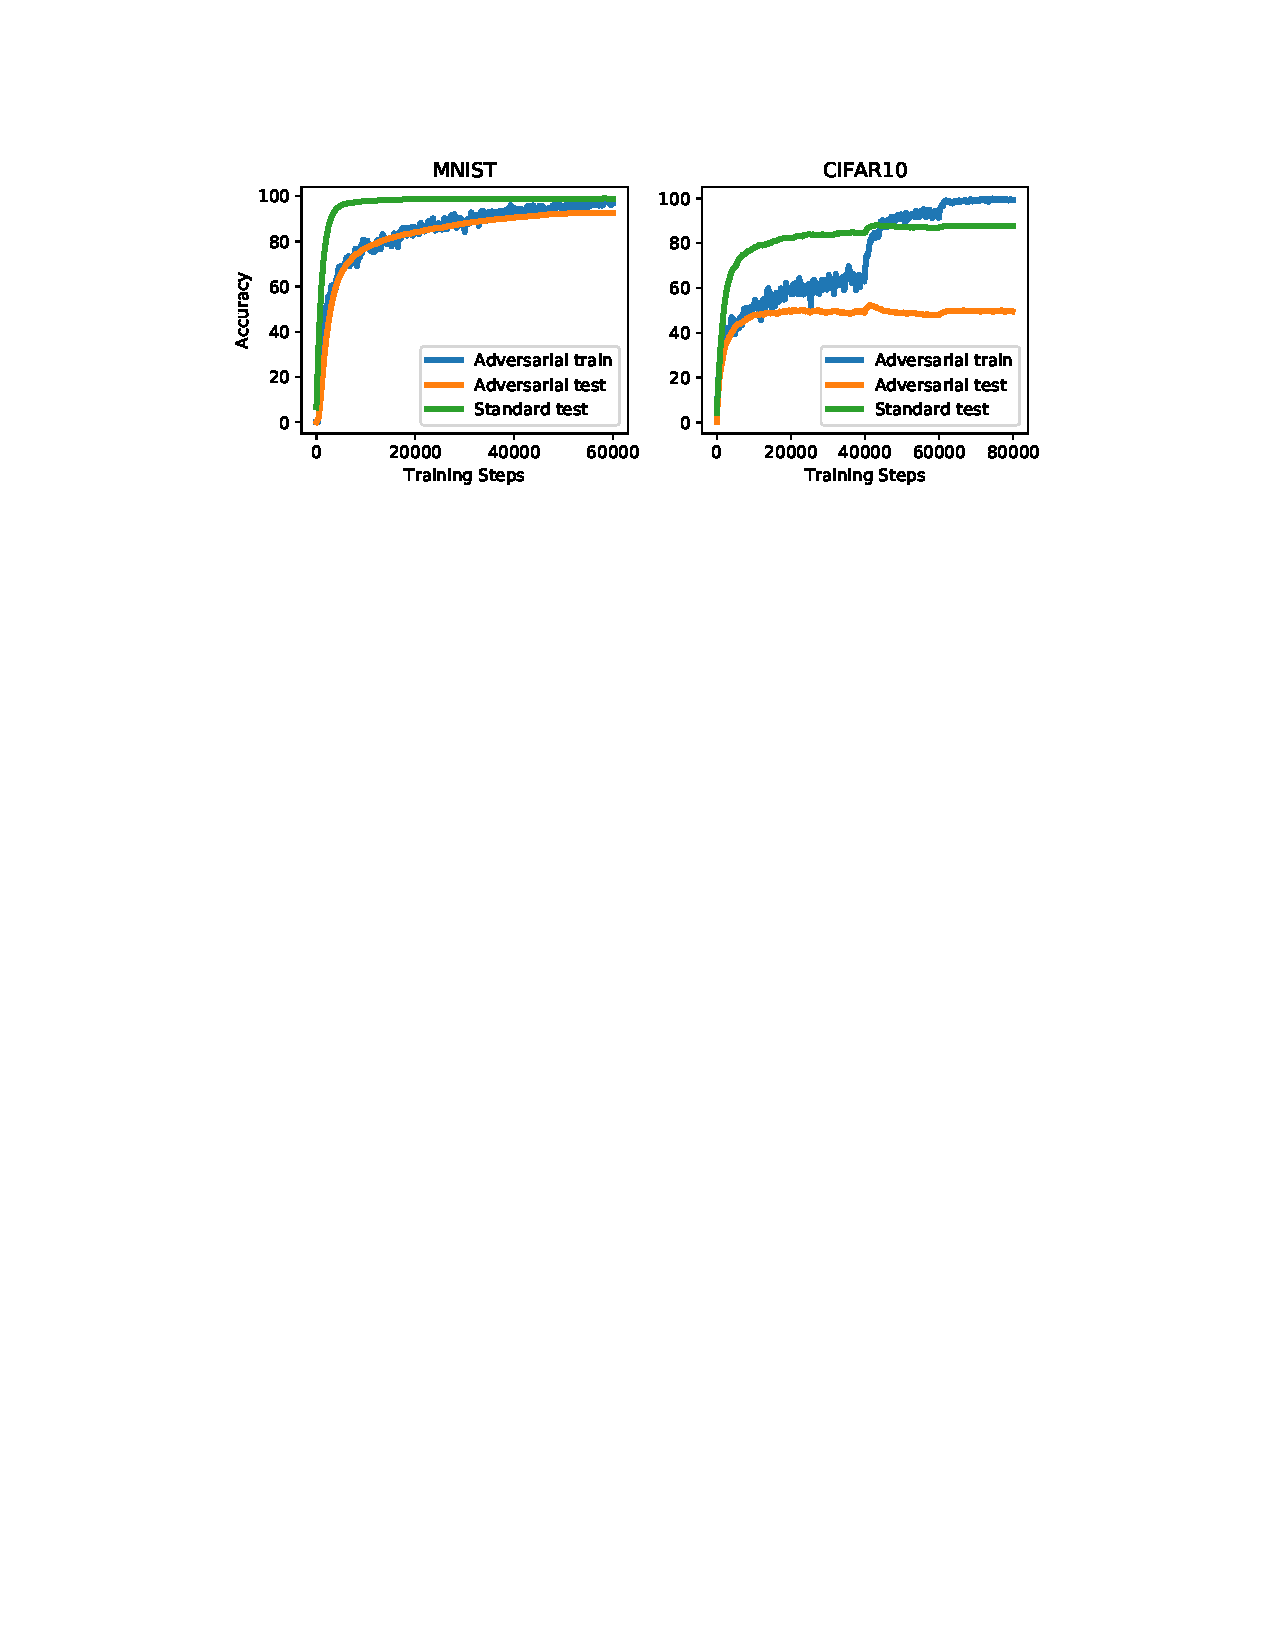
\includegraphics{fig/robust_optimization.pdf}
    \caption{在MNIST和CIFAR10上进行鲁棒优化(即对抗训练)的分类正确率}
    \label{fig:robust_optimization}
\end{figure}

许多的防御方法被提出来不久就被更强的攻击方法击败,唯有对抗训练(Adversarial training)这个简单且有效的方法经受住了时间的考验。对抗训练是将对抗样本作为训练集的一部分,让模型去学习,目的是使深度神经网络对未来(即测试时)样本的攻击具有更好的鲁棒性。Madry 等人\cite{madry2018towards}从鲁棒优化(Robust optimization) 的角度解释了对抗训练,表明对抗训练的过程是在每个训练样本的周围空间里寻找最坏的样本用以训练最优的分类器,并建议在对抗训练时使用一阶敌人(First-order adversary)作为自然且普适的安全性保证。

然而对抗训练本身的性能并不够理想。虽然通过合适的模型和适当的优化过程,对抗训练出来的模型可以将训练集样本较好地拟合,但是在测试集上的泛化性能却很差\cite{schmidt2018adversarially}。如\autoref{fig:robust_optimization}所示, 在 MNIST 上,对抗测试集精度接近对抗训练集精度(但还是有一些差距);在 CIFAR10 上,虽然模型在标准(非对抗)的测试集上有较高的精度,但在鲁棒精度上有一个非常大的鸿沟,即对抗测试集上的精度远低于对抗训练集上的精度。

对抗训练泛化能力的不足,暗示着我们应该为对抗训练设计更为有效的正则化方法,尤其是在深度神经网络过参数化的情况下。本文的主要任务,就是尝试结合度量学习的思想,利用相关的正则化方法,以提高对抗训练的泛化性能,并通过大量的实验进行有效性验证。